\chapter{Main part}
\section{Theory and background}
%HWSW Codesign theory

HW/SW Codesign is, as mentioned in the introduction, a topic that has risen up in modern times in relation to the gradual development of electronic gadgets of different kinds. The book "A practical introduction to Hardware/Software Codesign" \cite{IntroHWSW} has the following definition of HW/SW Codesign: 
\\\\
\begin{center}
\say{
Hardware/Software Codesign is the design of cooperating hardware components and software components in a single design effort.
}
\end{center}
\hfill\break
\hfill\break
\noindent
%Til forord eller liknende: HWSW-teori vil i denne rapporten være svært grunnleggende og mindre omfattende, da rapportens formål er å presentere en løsning på et problem heller enn teori om temaet. 
This definition provides a short and accurate description of what the topic is about, and will be used as basis for defining the topic in this report. Based on this definition, one could also say that HW/SW Codesign is the process of deciding which tasks of a system that should be implemented in hardware and software. 
From a designers' point of view, implementing designs in software might be considered the easiest approach to follow. The reason for this is that software is often considered easy and flexible in terms of editing, and when complemented with access to fast compilers as well as software libraries and computers that are easy to come by, choosing software over hardware seems obvious. According to sources however, the choice of implementing in HW or SW is a lot more subtle in practice, as it tends to depend on several other factors in addition to the ease of access and editing. These factors are based on both technological reasons as well as economical ones, and will be outlined in more detail in the following subsections. 
\\
\noindent
\subsection{Performance factor}
One of the most vital technological factors to consider when making the decision between HW and SW for a system design is the performance one expects to receive from the implementation. One can for instance consider performance to be the amount of work done per unit time, where a unit of work is defined as the processing of 1 bit of data, and time is measured in clock cycles or seconds. Figure \ref{HWSWPerformance}, derived from \cite{IntroHWSW}, gives an illustration of the variations in performance for hardware and software, based on these considerations. 

\begin{figure}[H]
    \begin{center}
        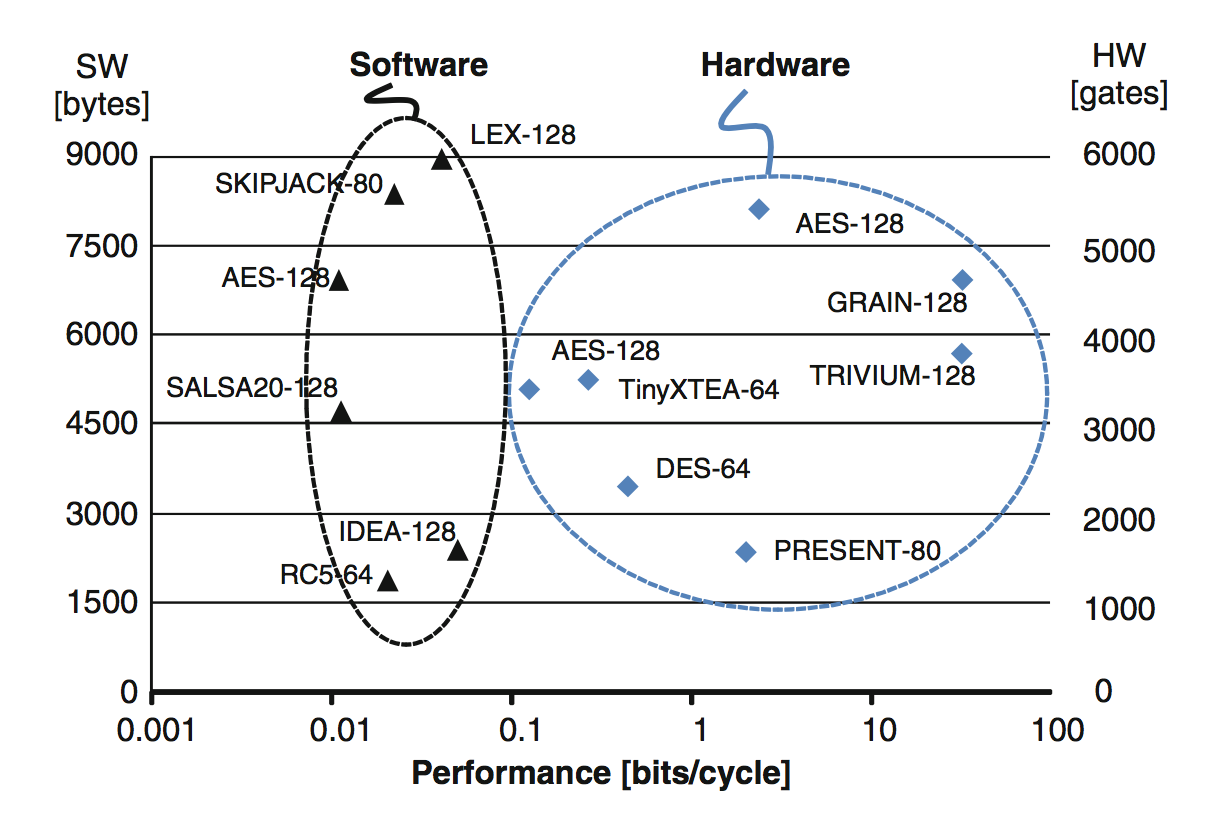
\includegraphics[scale=0.52]{Attachments/HWSWPerformance.png}
        \caption{Various cryptographic implementations in software and hardware proposed from the year 2003 to 2008 \cite{ReadingsHWSW}. }
        \label{HWSWPerformance}
    \end{center}
\end{figure}

\\\\
\noindent
The graph shows performance in bits per cycle. It demonstrates that, on average, hardware crypto-architectures
have a higher performance than embedded processors when one uses several different implementations for both HW and SW solutions. 
\\
Contrary to these results however, when one compares the clock frequency found in most hardware implementations to the clock frequency available in a processor executing a software implementation, the clock frequency in the processor may often outperform the one found in the hardware implementation. In this regard, the software implementation can achieve a higher performance than the hardware implementation simply because the processor performance outweighs the performance gained from the clock frequency and the parallel execution found in a corresponding hardware implementation. The decision between a hardware or software implementation based on performance therefore largely depends on the nature of the design task that is to be implemented, and in this sense whether the task is best suited to be executed in a parallel or a serial manner.  
\\
\noindent
\subsection{Energy efficiency}
Another technical factor to consider when choosing between hardware or software implementations is the aspect of energy efficiency or power consumption necessary for performing computations. Energy efficiency can be defined as the amount of useful work accomplished per unit of energy and is especially important to consider for portable battery operated applications. It is an established fact that increasing the energy efficiency results in a longer battery life, and this is intuitively a factor one seeks to have in portable battery operated applications. Figure \ref{Energyefficiency} gives an illustration of the amount of Gigabits possible to decrypt on each of the illustrated platforms, by using a single Joule of energy. 

\begin{figure}[H]
    \begin{center}
        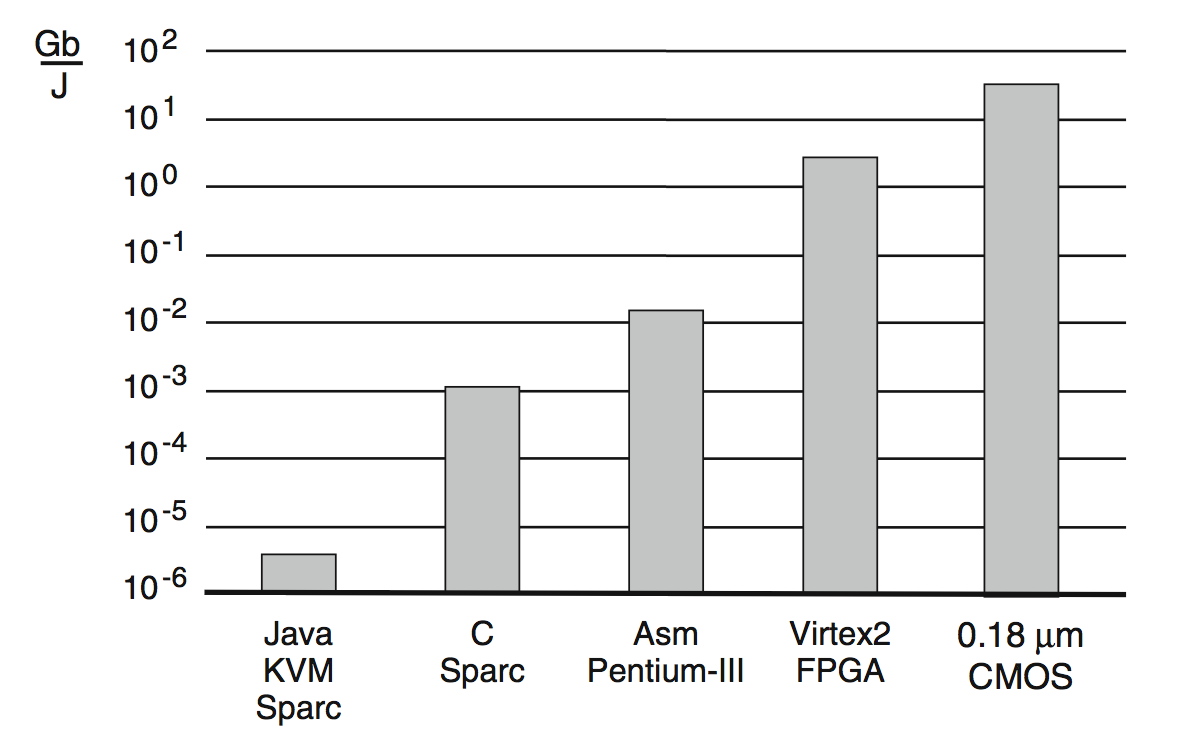
\includegraphics[scale=0.52]{Attachments/Energyefficiency.png}
        \caption{A particular encryption application used for different target platforms. }
        \label{Energyefficiency}
    \end{center}
\end{figure}

\noindent
The figure is meant to illustrate the amount of variation one can find in energy consumption for different target platforms. Despite the task being the same for all of the platforms, it can be seen from the figure that the amount of Gigabits decrypted for 1 Joule of energy varies over several orders of magnitude, which gives rise to a strong motivation for improving the energy efficiency as much as possible when designing a system. 
\\
\noindent
\subsection{Driving factors/Power density}
In the previous subsections it was outlined how a hardware implementation can usually outperform a software implementation and vice versa, and it was also pointed out how a system platform can have a power consumption that varies greatly in magnitude depending on the implementation used. This subsection will seek to give the full picture of what drives the hardware/software implementation decision by giving a short description of the other factors involved. 
\\
\noindent
As outlined previously, the performance and energy efficiency aspects of HW/SW Codesign generally favor a hardware design implementation over a software one because of the fixed and parallel nature of the former. Despite this fact, the design of modern electronic systems is characterized by the need to make a lot of trade-offs to achieve the optimal result for the given specification. Figure \ref{HWSWTradeoffs} displays a general overview of the trade-offs being made when choosing one over the other. 


\begin{figure}[H]
    \begin{center}
        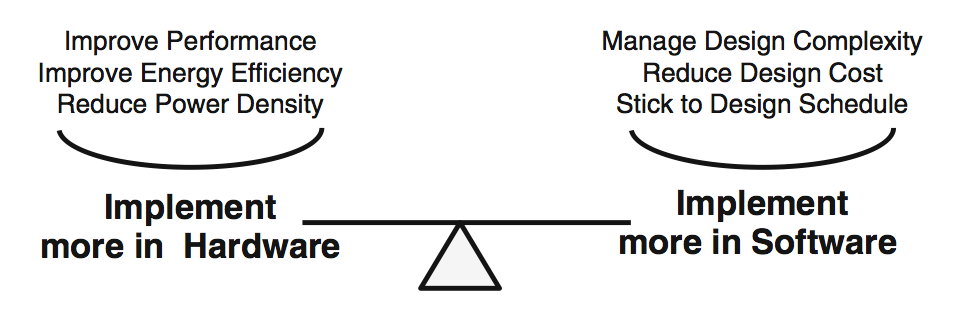
\includegraphics[scale=0.52]{Attachments/HWSWTradeoffs.png}
        \caption{The usual trade-offs needing to be made when choosing either a hardware- or a software implementation in the HW/SW Codesign philosophy. }
        \label{HWSWTradeoffs}
    \end{center}
\end{figure}
\hfill\break
\hfill\break
\noindent
Another factor involved in the implementation decision is therefore the power density or the power dissipation expected from a circuit. This factor is directly proportional to the clock frequency of a circuit, and thus applies to both hardware- and software implementations alike. In recent years the power density found in modern processors has reached a limit where modern cost-effective cooling technology can no longer keep up, and is unable to handle further increase in power. It is therefore believed that further performance increase cannot be achieved with increased clock frequency. The industry has therefore taken a large and fundamental shift towards parallel computer architectures. Examples of these architectures are Field Programmable Gate Arrays (FPGAs), Symmetric Multiprocessors (SMPs) and also dedicated processors for resource intensive tasks like graphics called Graphics Processing Units (GPUs).
\\
\noindent
\subsection{Design complexity}
The previous three subsections in this section have all presented factors for HW/SW implementations that favor hardware implementations. The factor of design complexity in modern systems however is one that is considered to be solved best with software, as flexible solutions that can easily be altered in the design without too much effort is favored over the fixed and hard coded nature of hardware implementations. This is evident when one looks at the complex attributes of modern electronic systems. To accommodate the design complexity in an optimal way, the aim is to make the implementation as flexible as possible, thus enabling the designer to alter the solution easily. The software is also used as a mechanism for creating higher levels of abstraction, to enable easier adjustments to future needs, and to solve problems with bugs. 
\\
\noindent
\subsection{Design cost}
Designing new chips is usually very expensive, which is why many hardware designers have begun making their chips programmable to enable them to be reused for different applications and multiple product generations. An example of this is the System on Chip (SoC) circuit, as well as FPGAs and others. 
\\
\noindent
\subsection{Shrinking design schedules}
It is usually always desirable to reduce the time needed to design a new electronic product. With new generations of electronic technology and applications continually bringing more complexity into the design, as well as replacing the older one quicker than before, the work load increases for the design engineer with each generation, which means that decreasing or shrinking the design schedules to complete the work in a shorter amount of time becomes necessary. In order to do this, the engineering teams attempt to work on multiple tasks at the same time, where hardware and software is then developed concurrently. As an example a software team will typically start development of the software to be run on the hardware as soon as the characteristics of the hardware is defined, and will begin before an actual prototype of the hardware is produced. 
\\
\noindent
\subsection{HW/SW Codesign space / Balancing}
With the previous subsections delving into the most prominent factors to consider for HW/SW Codesign, the art of making the optimal solution based on these factors is what the job of the design engineers is all about. The different trade-offs discussed also need to be put into the context of a design space. As can be derived from all the aforementioned factors, there are many different possible solutions for a design. The collection of all these solutions is called the HW/SW Codesign space, and is illustrated in a symbolic way in Figure \ref{HWSWDesignspace}. 


\begin{figure}[H]
    \begin{center}
        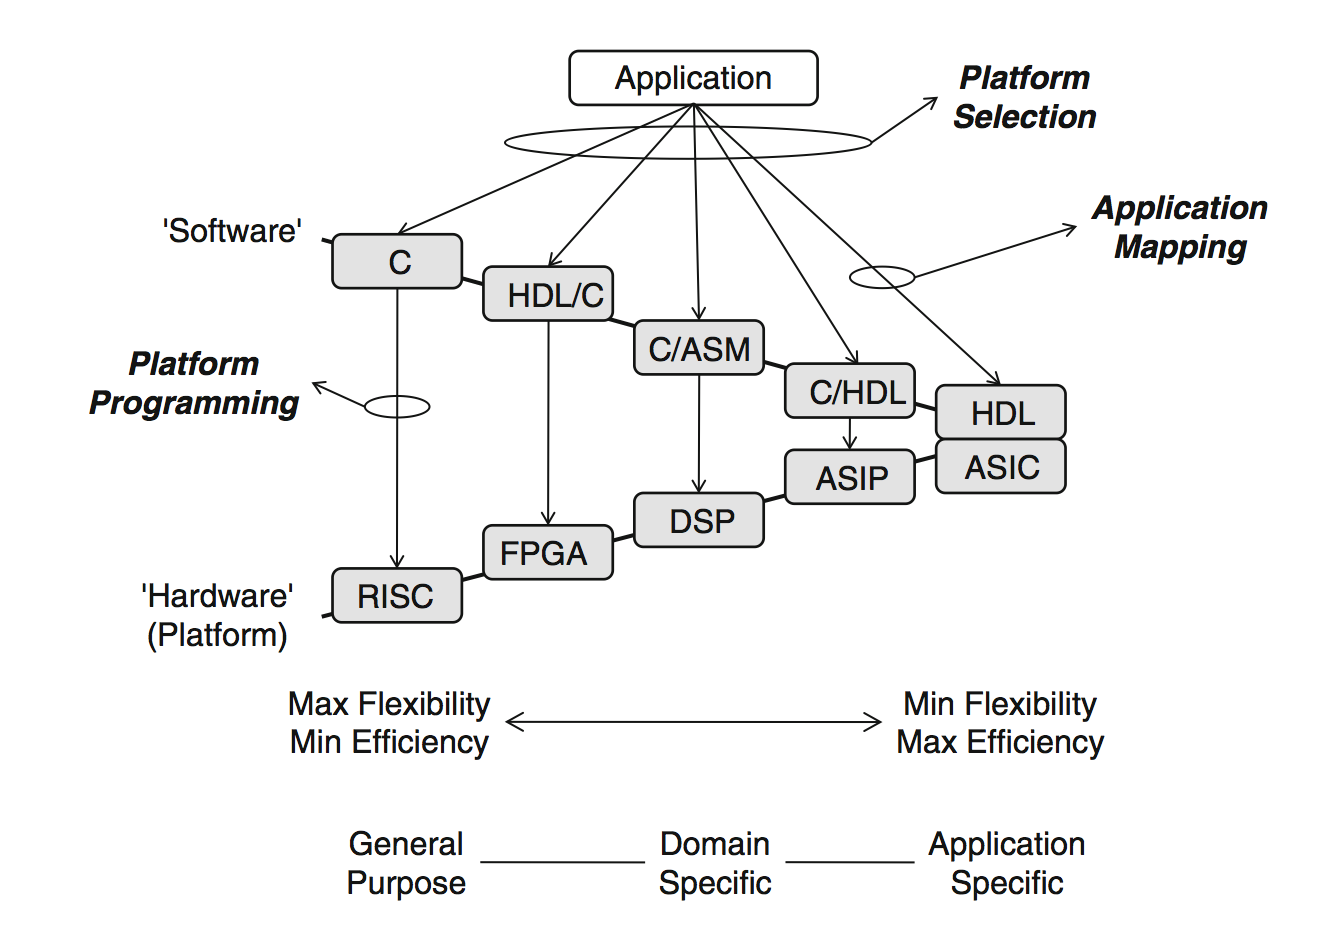
\includegraphics[scale=0.52]{Attachments/HWSWDesignspace.png}
        \caption{Illustration of the HW/SW Codesign space, outlined with the main activities. }
        \label{HWSWDesignspace}
    \end{center}
\end{figure}


\begin{comment}
In short terms, HW/SW Codesign seeks to increase the efficiency of electronic gadgets by improving the cooperation between the hardware and software of a system in the design phase. As mentioned in the introduction, this philosophy seeks to use the synergy normally found between hardware and software to improve the design of the system at an early stage. 
\\\\
\noindent
The book "A practical introduction to Hardware/Software Codesign" \cite{IntroHWSW} has the following definition for HW/SW Codesign: \\\\
\begin{center}
\say{
Hardware/Software Codesign is the design of cooperating hardware components
and software components in a single design effort.
}
\end{center}
\hfill\break
\hfill\break
\noindent
The nature of HW/SW Codesign can be considered as the process of finding the balance in the design for when to use hardware and when to use software to accomplish the tasks of a system. 
\\\\
\noindent
There are several key methods for carrying out the HW/SW Codesign philosophy in practice. One is to perform cosimulation of the hardware and software. 
\end{comment}





\section{Previous work}
Hva andre har gjort på feltet, f.eks. eksempler på andre designmetodikker. 

\section{Pedestrian Detection system}
This specialization project has used an application for a pedestrian detection system developed as part of the Tulipp project cite, and is used as basis for all the work and results outlined in this report. Since no further work to change the application was completed in this specialization project, the whole application in its entirety is the result of previous work performed by other project participants. The system used for the basis of this project's results consists of an online code repository that is meant to be compiled and run in the Linux computer operating system. Further details about the system are mentioned in the subsections below. 
\\\\

\subsection{Linux implementation}
%\addcontentsline{toc}{subsection}{\numberline{}6.1 - Linux implementation}
Something about how the project files are organized. Make files, Cmake, etc. \\\\

\subsection{System code}
%\addcontentsline{toc}{subsection}{\numberline{}6.2 - System code}
Some details about the languages used and basic notes on how they work. 
\\\\
\noindent
The previous code work completed for this application contains a great number of code files written in different languages, that are all used to make different test applications of the system run. %The test applications used as basis for this report is 
\\\\\\
\noindent
\textit{\color{red}\Big{Previous work:}\\
A description of what has been done before in this field. Also include background theory which is important to understand the work that is described later. Divide this into several chapters as needed. }\\
\clearpage




























\begin{comment}
\section{Previous work}
%\addcontentsline{toc}{section}{\numberline{}6 - Previous work}
This specialization project has used an application for a pedestrian detection system developed as part of the Tulipp project cite, and is used as basis for all the work and results outlined in this report. Since no further work to change the application was completed in this specialization project, the whole application in its entirety is the result of previous work performed by other project participants. The system used for the basis of this project's results consists of an online code repository that is meant to be compiled and run in the Linux computer operating system. Further details about the system is mentioned in the subsections below. 
\\\\

\noindent
\textit{\color{red}\Big{Previous work:}\\
A description of what has been done before in this field. Also include background theory which is important to understand the work that is described later. Divide this into several chapters as needed. }\\

\subsection*{6.1 - Linux implementation}
\addcontentsline{toc}{subsection}{\numberline{}6.1 - Linux implementation}
Something about how the project files are organized. Make files, Cmake, etc. \\\\

\subsection*{6.2 - System code}
\addcontentsline{toc}{subsection}{\numberline{}6.2 - System code}
Some details about the languages used and basic notes on how they work. 
\\\\
\noindent
The previous code work completed for this application contains a great number of code files written in different languages, that are all used to make different test applications of the system run. %The test applications used as basis for this report is 

\clearpage
\end{comment}

